\def\mytitle{PARALLELOGRAM}
\def\myauthor{VUNNAVA SRAVANI}
\def\contact{sravani21vunnava@gmail.com}
\def\mymodule{Future Wireless Communication (FWC)}
\documentclass[10pt, a4paper]{article}
\usepackage[a4paper,outer=1.5cm,inner=1.5cm,top=1.75cm,bottom=1.5cm]{geometry}
\twocolumn
\usepackage{graphicx}
\graphicspath{{./images/}}
\usepackage[colorlinks,linkcolor={black},citecolor={blue!80!black},urlcolor={blue!80!black}]{hyperref}
\usepackage[parfill]{parskip}
\usepackage{lmodern}
\usepackage{tikz}
	\usepackage{physics}
%\documentclass[tikz, border=2mm]{standalone}
\usepackage{karnaugh-map}
%\documentclass{article}
\usepackage{tabularx}
\usepackage{circuitikz}
\usetikzlibrary{calc}
\usepackage{amsmath}
\usepackage{amssymb}
\renewcommand*\familydefault{\sfdefault}
\usepackage{watermark}
\usepackage{lipsum}
\usepackage{xcolor}
\usepackage{listings}
\usepackage{float}
\usepackage{titlesec}
\providecommand{\mtx}[1]{\mathbf{#1}}
\titlespacing{\subsection}{1pt}{\parskip}{3pt}
\titlespacing{\subsubsection}{0pt}{\parskip}{-\parskip}
\titlespacing{\paragraph}{0pt}{\parskip}{\parskip}
\newcommand{\figuremacro}[5]{
    \begin{figure}[#1]
        \centering
        \includegraphics[width=#5\columnwidth]{#2}
        \caption[#3]{\textbf{#3}#4}
        \label{fig:#2}
    \end{figure}
}
\newcommand{\myvec}[1]{\ensuremath{\begin{pmatrix}#1\end{pmatrix}}}
\let\vec\mathbf
\lstset{
frame=single, 
breaklines=true,
columns=fullflexible
}

%\thiswatermark{\centering \put(181,-119.0){
\includegraphics[scale=0.13]{IIT_logo.png}} }
\title{\mytitle}
\author{\myauthor\hspace{1em}\\\contact\\FWC22012\hspace{6.5em}IITH\hspace{0.5em}\mymodule\hspace{6em}ASSIGN-5}
\date{}
\begin{document}
	\maketitle
	\tableofcontents
   \section{Problem}
  ABCD is a parallelogram and AP and CQ are
perpendiculars from vertices A and C on diagonal
BD . Show that \\
(i) $\Delta APB \cong \Delta$ CQD \\       
(ii) AP = CQ

	   % \includegraphics[scale=1.0]{diag_1.png}
   \section{Solution}
   \textbf{Theory:}\\
In parallelogram $ AB\: || \: CD$ and $ AD\: || \: BC$  \\
BD and AC are diagonals of the parallelogram which are also the transversals for $ AB\: || \: CD$\\
\textbf{To Prove:} $\Delta APB \cong\Delta$ CQD \\
$\angle {ABD}$ and $\angle {CDB}$ are equal since they are alternate interior angles\\
so $\angle {ABP}$ and $\angle {CDQ}$ are equal\\
$\angle {APB}$ and $\angle {CQD}$ are perpendicular angles\\

\begin{center}
$\therefore$ due to AAS (angle angle side ) rule\\
$\Delta APB \cong\Delta$ CQD   
\end{center}
\textbf{To Prove:}  AP = CQ\\
$\Delta APB \cong \Delta$ CQD   
\begin{center}
$\therefore$ AP = CQ    \\
Hence, Proved \\
\
\\
\end{center}

The input parameters for this construction are 
\begin{center}
\begin{tabular}{|c|c|}
	\hline
	\textbf{Symbol}&\textbf{Value}\\
	\hline
	b&6\\
	\hline
	r&5\\
	\hline
	$\theta$&$\frac{\pi}{3}$\\
	\hline
	A&$\
	\begin{pmatrix}
		0 \\
		0 \\
	\end{pmatrix}$%
	\\
	\hline
	B&$\
	\begin{pmatrix}
		b \\
		0 \\
	\end{pmatrix}$%
	\\
	\hline
	D&r$\
	\begin{pmatrix}
		cos\theta \\
		sin\theta \\
	\end{pmatrix}$%
	\\
	\hline
	C&B+D%
	\\
	\hline
\end{tabular}
\end{center}
\
\\
\
\\
\
\\
\
\\
\textbf{To Prove:} AP = CQ
		\begin{center}
		Points P and Q are drawn from the vertices A and C to the diagonal BD respectively\\
		The line equation for diagonal BD is x = B+$\lambda$m
		\\
		where m = B-D\\
		\
		\\
		then,\\
		\
		\\
		P = B - $\frac{m^T B}{\norm{m}^2}m$
	\\
	\
	\\
	\
	\\
	Q =  B - $\frac{m^T (C-B)}{\norm{m}^2}m$
	\\
	\end{center}
	
	distance between A and P is $\norm{A-P}$\\
	distance between C and Q is $\norm{C-Q}$\\
	if $\norm{A-P}$ =  $\norm{C-Q}$\\
	then AP = CQ..........(1)
	
	\textbf{To Prove:}  $\Delta APB \cong \Delta$ CQD\\
	to prove $\angle {APD}$ and $\angle {CQD}$ are 90$^{\circ}$\\
	m1 = A-P\\
	m2 = P-B\\
	if $\theta$ is the angle\\
	then cos$\theta$ = $\frac{m1^\intercal m2}{\norm{\vec{m1}}\norm{\vec{m2}}}$\\
	for $\theta$ = 90$^{\circ}$, cos$\theta$ = 0\\
	$\therefore m1^\intercal$ m2 = 0\\
	n1 = C-Q\\
	n2 = Q-D\\
	if $\theta$ is the angle\\
	then cos$\theta$ = $\frac{n1^\intercal n2}{\norm{\vec{n1}}\norm{\vec{n2}}}$\\
	for $\theta$ = 90$^{\circ}$, cos$\theta$ = 0\\
	$\therefore n1^\intercal$ n2 = 0\\
	\begin{center}
	if 	$m1^\intercal m2 = 0$  and $n1^\intercal n2$ = 0\\
	then, $\angle {APD}$ = $\angle {CQD}$ = 90$^{\circ}$..........(2)\\
	\end{center}
	to prove $\angle {ABP}$ and $\angle {CDQ}$ are equal\\
	m2 = P-B\\
	m3 = A-B\\
	let $\theta1$ be the $\angle {ABP}$\\
	then $\theta1 = \cos^-1\frac{\vec{m2} \cdot \vec{m3}}{\norm{\vec{m2}}\norm{\vec{m3}}}$\\
	n2 = C-D\\
	n3 = Q-D\\
	let $\theta2$ be the $\angle {CDQ}$\\
	then $\theta2 = \cos^-1\frac{\vec{n2} \cdot \vec{n3}}{\norm{\vec{n2}}\norm{\vec{n3}}}$\\
	\begin{center}
	 		if $\theta1 = \theta2$\\
	 		then $\angle {ABP} = \angle {CQD}$..........(3)
	\end{center}
	\begin{center}
$\therefore$ from (1),(2) and (3)
$\Delta APB \cong \Delta$ CQD
	\end{center}
	\
\\
\
\\
\
\\
The below python code realizes the above construction:	
\begin{lstlisting}
https://github.com/sravani21vunnava/sravani21vunnava/blob/main/Matrices_line/codes/matrix_line.py
\end{lstlisting}
 
\section{Construction}
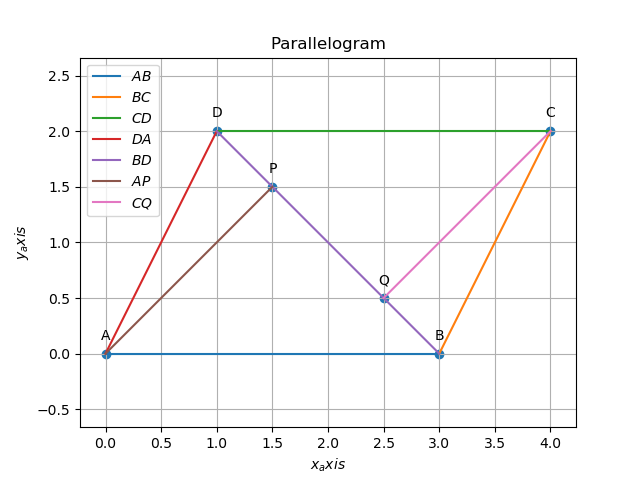
\includegraphics[scale=0.66]{matrix_line1.png}
 	
\bibliographystyle{ieeetr}
\end{document}